\documentclass[a4paper,runningheads]{llncs}
\usepackage[T1]{fontenc}
\usepackage{graphicx}
\usepackage{booktabs}
\usepackage{amsmath,amssymb}
\usepackage{microtype}
\usepackage{url}
\usepackage{xurl}
\AtBeginDocument{\renewcommand{\doi}[1]{\url{https://doi.org/#1}}}
\usepackage{cite}
\usepackage{xcolor}

\InputIfFileExists{generated/macros.tex}{}{}
% Fallbacks shown only if a result file is missing.
\providecommand{\PermMaxCarf}{??}\providecommand{\NPerm}{??}\providecommand{\PermPCarf}{??}

\newcommand{\logit}{\operatorname{logit}}
\newcommand{\clip}{\operatorname{clip}}

\pdfinfoomitdate=1
\pdftrailerid{}
\pdfsuppressptexinfo=-1
\begin{document}
\title{CARF: Bounded Anchored Fusion for Multimodal Prediction with Unreliable Modalities}
\titlerunning{CARF: Bounded Anchored Fusion}
\author{Anonymous Authors}
\authorrunning{Anonymous Authors}
\institute{Anonymous Institution}
\maketitle

\begin{abstract}
In clinical prediction, some inputs are recorded for every patient, while others may be missing, measured only in some cohorts, or silently wrong, e.g., after a specimen swap. We propose Clinical-Anchored Residual Fusion (CARF), which keeps the logit of an always-available clinical model as an anchor and lets each optional modality move it only within a log-odds budget. An \emph{anchor-verification gate} scales each optional contribution by the posterior probability that the sample belongs to the patient, estimated from auxiliary heads that predict hormone-receptor and HER2 status. With exact mask handling and a convex objective over missingness, sample swaps, and extreme outputs, CARF keeps exact fallback to the anchor and a per-patient bound on the change of the prediction. For pathological complete response, we combine a treatment-aware anchor with expression, MRI, and a proteomic modality available for only part of the development cohort. On \NDev{} I-SPY2 patients, CARF reaches an AUROC of \IntCarfTwo{}, statistically indistinguishable from unconstrained fusion, and fusion baselines that receive the same gate are as robust internally. On the external I-SPY1 cohort, the bound matters: CARF's worst-case AUROC over modality failures (\ExtWorstCarfTwo{}) exceeds that of every gated or ungated baseline except a gated robust offset model, with paired intervals excluding zero, and no prediction moves by more than \MaxDispCarfTwo{} logits from the clinical one.
\keywords{Multimodal learning \and Missing modalities \and Robust fusion \and Sample verification \and Bounded influence}
\end{abstract}

%======================================================================
\section{Introduction}

Multimodal learning combines heterogeneous sources of information about the same individual \cite{baltrusaitis2019}. In clinical applications, some inputs are cheap and recorded for every patient, whereas others are optional, site-dependent, available only in some cohorts, or of unknown quality. A fusion model trained on complete data can depend on an optional modality to a degree that is not safe when it is absent or wrong. Stacking \cite{wolpert1992} and learned gates may give a large weight to an expert that is accurate on the training cohort, and confidence scores do not remove this risk: after a sample swap, the expert output is plausible and confident but uninformative.

We study this problem for the prediction of pathological complete response (pCR), i.e., no invasive cancer at surgery after neoadjuvant chemotherapy, in the public I-SPY1 \cite{esserman2012} and I-SPY2 \cite{wolf2022ispy} breast cancer trials. Clinical variables such as hormone-receptor (HR) and HER2 status and the planned regimen are available for every patient, whereas pretreatment gene expression, dynamic contrast-enhanced MRI, and reverse-phase protein arrays (RPPA) are optional; RPPA was measured for \NRppa{} of the \NDev{} I-SPY2 patients and for none of the I-SPY1 patients.

We propose Clinical-Anchored Residual Fusion (CARF), which treats the always-available modality as an anchor and restricts how far the optional modalities can move the prediction: (i) a bounded, mask-aware fusion rule for any number of optional modalities that falls back exactly to the anchor; (ii) an \emph{anchor-verification gate}, in which the posterior probability that an optional sample matches the clinical HR/HER2 record scales its residual without weakening any guarantee; (iii) a convex objective over all availability patterns and failures including sample swaps, with the budget chosen by inner cross-validation; and (iv) an evaluation that separates the gate from the bound by giving every baseline the same gate, with semi-realistic specimen mix-ups and confidence intervals for all robustness claims.

%======================================================================
\section{Related Work}

ModDrop \cite{neverova2015} and related training schemes \cite{ma2021smil} make fusion models tolerate absent modalities by dropping them during training, but do not limit how much a present, corrupted modality can change a prediction. Several approaches weight experts by an estimated quality: QA-MoE \cite{sun2026} separates quality estimation from expert routing for clinical prediction with noisy and missing modalities, QMF \cite{zhang2023qmf} derives generalization guarantees for uncertainty-weighted late fusion, and Moon et al.~\cite{moon2026} question whether such scores change downstream decisions. Such scores come from the modality itself and cannot detect a confident expert applied to a swapped sample. Offset logistic regression is the standard way to update a clinical model with new predictors \cite{janssen2008}, and UCMR-Net \cite{tang2026} adds adaptive residuals to a text anchor for sentiment prediction, without bounding the total correction. Our fitting objective is related to distributionally robust optimization \cite{sagawa2020}, with environments that are availability patterns and failures of the optional experts. CARF instead bounds the correction by construction and verifies each optional sample against variables recorded for every patient.

%======================================================================
\section{Approach}

Consider a binary outcome $y$ and experts that are each trained on one modality. The anchor expert outputs a probability $p_C$ for every patient; the optional experts $j=1,\dots,K$ output probabilities $p_j$ with availability indicators $m_j\in\{0,1\}$. Let $a=\logit(p_C)$ be the anchor logit and $d_j=\logit(p_j)-a$. We seek a fusion rule that (i) returns $a$ exactly when all optional inputs are absent, (ii) keeps the fused logit within a known distance of $a$, (iii) reduces the contribution of an optional sample that is inconsistent with the patient's record, and (iv) is fitted with a procedure that accounts for missing and failing optional inputs.

\subsection{Anchored residual fusion}

For each optional expert, CARF clips the logit difference to $[-B,B]$, i.e., $r_j=\clip(d_j,-B,B)$, and scales it by three context functions with values in $[0,1]$: $h_{j0}=1$, $h_{j1}=e^{-|d_j|}$, which reduces the correction when the expert strongly disagrees with the anchor, and $h_{j2}=1-H(p_j)/\log2$, with the binary entropy $H$, which allows a different correction for confident experts. With the verification gate $g_j\in[0,1]$ defined below, the fused logit is
\begin{equation}
 z_\theta = a + \sum_{j=1}^{K}\sum_{k=0}^{2}\theta_{jk}\, m_j\, g_j\, h_{jk}\, r_j,
 \qquad \theta_{jk}\ge 0,\qquad \sum_{j,k}\theta_{jk}\le 1 .
 \label{eq:carf}
\end{equation}
A missing modality contributes zero, so that absence is represented by the mask and never by an imputed probability; since the coefficients are nonnegative, CARF can reduce the influence of an optional expert but cannot reverse its direction (Fig.~\ref{fig:architecture}).

\begin{figure}[t]
\centering
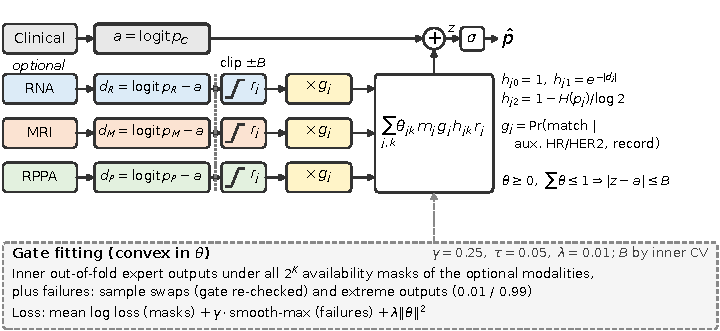
\includegraphics[width=0.88\linewidth]{figures/fig_architecture.pdf}
\caption{CARF with a clinical anchor (C) and optional RNA (R), MRI (M), and RPPA (P) experts. Each optional expert contributes a clipped residual $r_j$ relative to the anchor logit $a$, multiplied by its verification gate $g_j$, its mask $m_j$, and context functions $h_{jk}$, and weighted by $\theta\ge0$ with $\sum\theta\le1$. Auxiliary heads predict HR/HER2 from each optional modality; $g_j$ = posterior probability that the sample matches the clinical record.}
\label{fig:architecture}
\end{figure}

\paragraph{Anchor-verification gate.} The anchor contains variables that are also reflected in the optional modalities: HR and HER2 status are recorded clinically and are strongly associated with the expression of the corresponding genes and proteins. For each optional modality $j$, we train auxiliary logistic heads $q_{jt}$ that predict the anchor variables $t\in\{\mathrm{HR},\mathrm{HER2}\}$ from the modality, without the outcome. For a patient with recorded values $c_t$, let $\ell_j=\prod_t q_{jt}^{c_t}(1-q_{jt})^{1-c_t}$ be the likelihood of the record under the patient's own sample, and let $\bar\ell_j$ be the same quantity averaged over the samples of the training patients, i.e., the likelihood if the sample came from a random other patient. The gate is the posterior probability of a match,
\begin{equation}
 g_j = \Pr(\text{match}\mid q_j, c) = \frac{\pi\,\ell_j}{\pi\,\ell_j+(1-\pi)\,\bar\ell_j},
 \label{eq:gate}
\end{equation}
with a prior $\pi$ that mix-ups are rare ($\pi=0.95$). The gate needs no labels beyond the anchor and is computed per patient at prediction time. If a modality carries no information about the anchor variables, then $\ell_j\approx\bar\ell_j$ and $g_j\approx\pi$ for every patient, so an uninformative check leaves the fusion unchanged up to a constant that the coefficients $\theta$ absorb. Unrecorded anchor variables are skipped.

\subsection{Properties}

Let $b_j=B\sum_k\theta_{jk}$ be the budget of modality $j$ and $b=\sum_jb_j\le B$ the total budget. Since every summand of Eq.~\eqref{eq:carf} satisfies $|m_jg_jh_{jk}r_j|\le B$ and depends only on the anchor and on modality $j$, three properties hold for any values of the optional inputs. \emph{Fallback:} if all $m_j=0$, then $z_\theta=a$. \emph{Bounded displacement:} $|z_\theta-a|\le b$, and hence $|\hat p-p_C|\le b/4$. Replacing, removing, or swapping the sample of modality $j$ alone changes $z_\theta$ by at most $2b_j$. \emph{Ranking certificate:} two patients whose anchor logits differ by more than $2b$ keep their anchor ordering for any optional inputs. All statements also hold with the sharper budget $b^*_j=B\theta_{j0}+\kappa\theta_{j1}+B\theta_{j2}$, with $\kappa=\max_{t\le B}te^{-t}$. The verification gate can only shrink the residuals, so it does not weaken any bound.

\subsection{Convex robust gate fitting}

The gate coefficients $\theta$ are fitted on out-of-fold expert and auxiliary predictions obtained by five-fold cross-fitting within the training set. Let $L_e(\theta)$ be the mean logistic loss of $z_\theta$ in environment $e$. The set $\mathcal M$ contains all $2^K$ availability patterns of the optional modalities, and the set $\mathcal F$ contains failure environments: for each optional modality, four sample swaps, in which the modality's outputs are permuted among the patients who have it and the verification gate is recomputed against the receiving patient's record, and two extreme outputs ($0.01$ and $0.99$). We minimize
\begin{equation}
 \min_{\theta\ge0,\ \mathbf 1^\top\theta\le1}\;
 \frac1{|\mathcal M|}\sum_{e\in\mathcal M}L_e(\theta)
 +\gamma\,\tau\log\Big(\frac1{|\mathcal F|}\sum_{e\in\mathcal F}e^{L_e(\theta)/\tau}\Big)
 +\frac\lambda2\|\theta\|_2^2 .
 \label{eq:objective}
\end{equation}
The second term is a smoothed maximum over failures. For fixed expert and auxiliary outputs, $z_\theta$ is linear in $\theta$, so each $L_e$ is convex, the problem is strictly convex over a polytope for $\lambda>0$, and we solve it with sequential least-squares programming. We fix $\gamma=0.25$, $\tau=0.05$, and $\lambda=0.01$ and choose $B\in\{1,1.5,2,3\}$ by inner five-fold cross-validation of the held-out value of the objective, without the penalty; no hyperparameter is chosen on an evaluation cohort.

%======================================================================
\section{Experiments}

\subsection{Experimental setup}

\paragraph{Data.} We use \NDev{} I-SPY2 patients (\NDevPos{} with pCR) for development and \NExt{} I-SPY1 patients (\NExtPos{} with pCR) with complete expression and MRI as the external cohort, as well as 87 further I-SPY1 patients with a naturally missing modality and 409 patients of the independent cohort GSE25066 \cite{hatzis2011} without its I-SPY1 samples. Expression is restricted to the \NGenes{} genes shared by both platforms and rank-normalized within each patient; MRI features are computed within the tumor masks of the BreastDCEDL release \cite{fridman2026} of the TCIA collections \cite{tciaispy1,tciaispy2}. RPPA (\NRppaFeat{} proteins and phosphoproteins \cite{wolf2022ispy}) is missing for 25\% of the development cohort and for the whole external cohort.

\paragraph{Experts.} The anchor is \emph{treatment-aware}: in addition to age, HR, and HER2 status, it contains four indicators of the planned therapy class (anti-HER2 antibody, immunotherapy, platinum, and HER2 tyrosine-kinase inhibitor), which are known before treatment starts and are recorded for every patient; in I-SPY1, only trastuzumab is used. Each expert is a class-balanced logistic regression with fixed hyperparameters: on the seven anchor variables; on 250 genes selected within each training set by variance and an ANOVA test; on \NMriFeat{} intensity, shape, kinetic, and texture MRI features; and on the RPPA features ($C=0.01$), fitted on the patients who have them. The auxiliary heads are unweighted logistic regressions on the same inputs (50 ANOVA-selected genes for RNA). All preprocessing is fitted within each training partition.

\paragraph{Protocol.} Internal evaluation uses five repeats of stratified five-fold cross-validation on I-SPY2, in which inner cross-fitting produces the expert predictions used to fit every fusion model; external models are fitted on all of I-SPY2. I-SPY1 labels are not used to fit models, but external performance informed exploratory RNA feature-set screening, so I-SPY1 is not an untouched test set.

\paragraph{Baselines.} All fusion models receive the same expert outputs: the mean of available probabilities; stacking \cite{wolpert1992}; mask-stacking, i.e., stacking with availability indicators trained on all availability patterns; offset logistic regression with the anchor logit as offset \cite{janssen2008}, and its version trained with a robust objective over extreme outputs (robust offset LR); and a ModDrop-style MLP \cite{neverova2015} on probabilities and indicators, trained on all patterns with its architecture chosen by inner cross-validation. To separate the gate from the bound, every baseline is also fitted to \emph{gated} experts, $\logit\tilde p_j=a+g_j(\logit p_j-a)$, with the gate of Eq.~\eqref{eq:gate}.

\paragraph{Metrics and stress tests.} All models are frozen before any failure is simulated. For each optional modality, we remove it (\emph{missing}) or swap its sample among the patients who have it (\emph{swap}, 5 realizations per internal fold and 30 externally); a swap carries the auxiliary outputs along, as a real specimen exchange would. For the specimen-based modalities, we also simulate three \emph{semi-realistic mix-ups} on 20\% of the samples: an \emph{offset}, in which a contiguous run in GEO accession order is assigned to the next patient, as after a skipped well; a \emph{batch} swap within the processing batch (expression platform and normalization, or RPPA array); and a \emph{subtype} swap among patients with the same HR/HER2 status, which the gate cannot detect (all samples). Externally, we also corrupt the inputs of the frozen experts (50\% of the genes removed, 25\% shifted by two log-ratio units, MRI noise of one training SD, or 60\% of the MRI features removed; 30 realizations each). We report the AUROC, its average over the missing and swap scenarios (six internally, four externally), and its worst case over the intact inputs and these failures. Internal intervals use the corrected resampled $t$-test \cite{nadeau2003} over the 25 folds, and external intervals 2{,}000 paired patient bootstrap resamples with realizations held fixed. Refitting the whole pipeline on permuted I-SPY2 labels gives an external AUROC of at most \PermMaxCarf{} for CARF over \NPerm{} permutations ($p=\PermPCarf$).

\subsection{Discrimination and calibration}

\begin{table}[t]
\centering
\caption{Discrimination on intact inputs and under modality failure. Internal: mean over 25 outer folds on I-SPY2. Fail.\ avg: mean AUROC over missing and swapped RNA, MRI, and RPPA internally (RNA and MRI externally). Worst: minimum over intact inputs and these failures; 95\% CI for CARF (paired intervals for all comparisons in the supplement). $\max|z-a|$: largest change of the logit from the clinical anchor over all external scenarios.}
\label{tab:main}
\setlength{\tabcolsep}{3pt}
\resizebox{\linewidth}{!}{\InputIfFileExists{generated/tab_main.tex}{}{\textit{[table pending]}}}
\end{table}

On intact inputs (Table~\ref{tab:main}), CARF reaches an internal AUROC of \IntCarfTwo{} (SD over repeats \IntCarfTwoSd{}), compared with \IntMean{} for the mean, \IntStack{} for stacking, and \IntMaskStack{} for mask-stacking; none of these differences is significant (CARF minus stacking \DIntIntactStack{}, $p\PIntIntactStack$). Externally, CARF reaches \ExtCarfTwo{}, and the paired intervals against all fusion baselines include zero (e.g., $[\DExtStackLo,\DExtStackHi]$ against stacking), whereas the interval against the clinical expert is $[\DExtClinicalLo,\DExtClinicalHi]$. The gate changes the intact AUROC of any baseline by at most \GateIntactDropInt{} internally and \GateIntactDropExt{} externally. Internal Brier scores are similar (CARF \IntBrierCarfTwo{}, stacking \IntBrierStack{}; supplementary material); these class-balanced models overestimate prevalence and were not recalibrated. The treatment-aware anchor and the partially available RPPA modality mainly benefit the bounded rule: with an age/HR/HER2 anchor and only expression and MRI, CARF is \DesGapVOne{} below stacking internally (\DesVOneCarfTwo{} versus \DesVOneStack{}), and with both changes the gap shrinks to \DesGapFinal{} (supplementary material).

\subsection{Modality failure}
\label{sec:stress}

\emph{Internal cohort.} Under the six internal failures (Table~\ref{tab:main}), CARF reaches a failure average of \IntFailCarfTwo{} (95\% CI $[\IntFailCarfTwoLo,\IntFailCarfTwoHi]$) and a worst case of \IntWorstCarfTwo{} $[\IntWorstCarfTwoLo,\IntWorstCarfTwoHi]$. Its worst case is above that of the mean ($[\DIntWorstMeanLo,\DIntWorstMeanHi]$), but every other paired interval includes zero, e.g., $[\DIntWorstStackLo,\DIntWorstStackHi]$ against stacking. The gate explains this: the gated baselines reach failure averages of up to \IntFailGatedMean{} and worst cases of up to \IntWorstGatedOffsetLr{}. A swapped RNA sample is the most harmful failure (per-scenario results in the supplementary material): the mean drops to \IntRnaSwapMean{} and stacking to \IntRnaSwapStack{}, whereas CARF keeps \IntRnaSwapCarfTwo{}.

\emph{External cohort.} Here the RNA expert is the strongest optional expert, and the bound matters. CARF has a failure average of \ExtFailCarfTwo{} $[\ExtFailCarfTwoLo,\ExtFailCarfTwoHi]$ and a worst case of \ExtWorstCarfTwo{} $[\ExtWorstCarfTwoLo,\ExtWorstCarfTwoHi]$. Its worst case exceeds that of every ungated baseline and of every gated baseline except gated robust offset LR (\ExtWorstGatedRobustOffsetLr{}, $[\DExtWorstGatedRobustOffsetLrLo,\DExtWorstGatedRobustOffsetLrHi]$), e.g., by $[\DExtWorstGatedMaskStackLo,\DExtWorstGatedMaskStackHi]$ against gated mask-stacking. Its failure average cannot be distinguished from those of mask-stacking, the ModDrop MLP, robust offset LR, and their gated versions. Removing the gate from CARF changes the external worst case by only $[\DExtWorstCarfTwoNoGateLo,\DExtWorstCarfTwoNoGateHi]$: externally, the bound and the robust objective, not the gate, carry the robustness. Under input-level corruption, CARF remains above the clinical expert (\ExtClinical{}) in all scenarios, e.g., \InpRnaDropoutFiveZeroCarfTwo{} with half of the genes missing, compared with \InpRnaDropoutFiveZeroStack{} for stacking.

\begin{table}[t]
\centering
\caption{AUROC under semi-realistic specimen mix-ups of 20\% of the samples (offset in accession order; swap within processing batch) and under swaps within HR/HER2 subtype (all samples). Internal: mean over 25 folds with 5 realizations; external: 30 realizations.}
\label{tab:mixup}
\setlength{\tabcolsep}{3pt}
\resizebox{\linewidth}{!}{\InputIfFileExists{generated/tab_mixup.tex}{}{\textit{[table pending]}}}
\end{table}

\emph{Semi-realistic mix-ups.} Offsets and batch swaps of 20\% of the samples cost every fusion model at most \MixMaxLossInt{} internal AUROC relative to its intact value, so that the internal ranking essentially follows the intact one (Table~\ref{tab:mixup}). Externally, CARF and the gated robust offset model lose the least (\MixExtRnaOffsetCarfTwo{} and \MixExtRnaOffsetGatedRobustOffsetLr{} under an RNA offset, versus \MixExtRnaOffsetGatedStack{} for gated stacking). Subtype swaps, which the gate cannot detect, are more harmful: externally, CARF keeps \MixExtRnaSubtypeswapCarfTwo{}, close to CARF without gate (\MixExtRnaSubtypeswapCarfTwoNoGate{}) and gated robust offset LR (\MixExtRnaSubtypeswapGatedRobustOffsetLr{}) and above the other models, whereas internally ungated offset LR (\MixIntRnaSubtypeswapOffsetLr{}) is above CARF (\MixIntRnaSubtypeswapCarfTwo{}).

\begin{figure}[t]
\centering
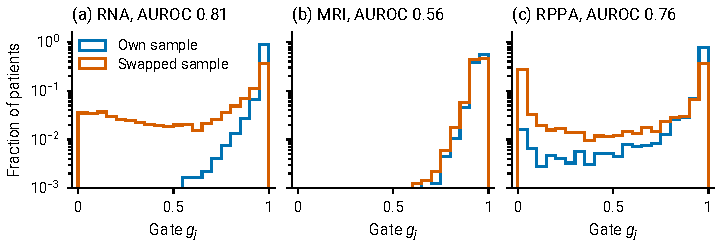
\includegraphics[width=0.9\linewidth]{figures/fig_gate.pdf}
\caption{Verification gate $g_j$ for patients with their own sample (blue) and with a swapped sample (orange), pooled over the internal test folds. The AUROC measures how well the gate separates the two.}
\label{fig:gate}
\end{figure}

\emph{Gate.} Fig.~\ref{fig:gate} shows that the gate separates own from swapped samples for the molecular modalities (AUROC \GateAucRna{} for RNA and \GateAucRppa{} for RPPA) and not for MRI (\GateAucMri{}), whose features barely reflect receptor status. The mean gate of own samples is \GateTrueRna{} for RNA and \GateTrueRppa{} for RPPA, so that the gate rarely reduces a correct contribution; for swapped samples, it falls below 0.5 in \GateLowRna\% (RNA) and \GateLowRppa\% (RPPA) of the cases. Within CARF, removing the robust term lowers the RNA-swap AUROC to \IntRnaSwapCarfTwoNoRobust{} internally and \ExtRnaSwapCarfTwoNoRobust{} externally (supplementary material).

\subsection{Naturally missing modalities}
\label{sec:natural}

In I-SPY1, we apply the frozen models with true masks to \NatPartialN{} further patients with only expression or MRI. Across patients with at least one optional modality, CARF reaches \NatAllCarfTwo{} (clinical: \NatAllClinical{}); in the partial subgroup it trails the clinical model (\NatPartialCarfTwo{} vs. \NatPartialClinical{}), so a single optional modality adds no discrimination.

\emph{Independent cohort.} On GSE25066 (\GseN{} patients), we apply the I-SPY2 pipeline, refitting RNA on I-SPY2 using only shared genes; no GSE25066 labels are used. CARF matches the clinical model on intact inputs (\GseIntactCarfTwo{} vs. \GseIntactClinical{}) and remains at that level under RNA swap (\GseRnaSwapCarfTwo{}; details in the supplement).

\subsection{Budget and robustness trade-off}

The inner cross-validation chooses $B=1.5$ or $2$ (\BudgetList{} of 25 folds). A fixed $B=1$ or training without swaps gives similar robustness (external RNA swap \ExtRnaSwapCarfTwoBOne{} and \ExtRnaSwapCarfTwoNoSwap{}) at a lower internal accuracy (\IntCarfTwoBOne{} and \IntCarfTwoNoSwap{}). The unbounded rule is the most accurate externally (\ExtCarfTwoUnbounded{}) but less robust (RNA swap \ExtRnaSwapCarfTwoUnbounded{}) and without guarantee (displacement \MaxDispCarfTwoUnbounded{}). The largest displacement of CARF from the anchor over all external scenarios is \MaxDispCarfTwo{} logits, below the sharp budget of the RNA and MRI terms (\SharpBudgetExt{}), whereas the other fusion models, gated or not, move predictions by up to \MaxDispGatedOffsetLr{} logits; when every optional modality is removed, CARF returns the clinical prediction exactly.

%======================================================================
\section{Conclusions}

We introduced bounded anchored fusion, an anchor-verification gate, and a convex objective that includes sample swaps. CARF matches unconstrained fusion on intact inputs and guarantees exact fallback and bounded prediction changes.

CARF guarantees stability, not accuracy; it does not improve intact-input discrimination or help small naturally missing subgroups. The gate cannot detect within-subtype swaps or anchor failures, and HR/HER2 do not verify MRI. Mix-ups are simulated, and I-SPY1 performance informed exploratory RNA feature-set screening, so its results are not an untouched validation. Future work should evaluate the method on documented mix-ups and verify imaging with additional recorded variables.

\bibliographystyle{splncs04}
\bibliography{references}
\end{document}
